\chapter{Definici\'on Empresa de Desarrollo de Software}
\section{Constituci\'on de la Empresa}
\subsection*{Nombre de la Empresa}
SOFBORe
\subsection*{Raz\'on Social}
Software BORe, S.A.S
\subsection*{Actividad Econ\'omica}
Empresa de servicios dirigidos a actividades de información y apoyo administrativo.

\section{Misi\'on}
Desarrollar software de buena calidad que permita la solución de problemas
encontrados en las PYMES de manera integral, adaptado a las necesidades de cada una 
de estas empresas.

\section{Visi\'on}
Estar comprometidos con los clientes de forma transparente y eficaz para convertirnos
en su socio de confianza, así mismo ser una empresa de referencia que camine con el 
cambio de la tecnología y la sociedad.

\section{Objetivos}
\begin{itemize}
\item Analizar los distintos problemas presentados por nuestros clientes para concebir 
las posibles óptimas soluciones para ofrecer a los mismos.
\item Desarrollar y comercializar software diseñado para facilitar y automatizar 
diferentes tareas en las PYMES.
\item Generar productos de buena calidad y un aceptable nivel competitivo.
\end{itemize}

\section{Metas}
\begin{itemize}
\item Anticiparse a las necesidades de los clientes teniendo en cuenta la posibilidad de 
clientes que puedan llegar a consultoría.
\item Entablar una relación de confianza y lealtad entre la empresa y los clientes PYMES.
\item Crear Software que ayude a convertir a clientes potenciales en clientes constantes 
de la empresa.
\item Ser lo más transparente en el desarrollo y la entrega de los productos.
\end{itemize}

\section{Pol\'iticas}
Es nuestro compromiso ofrecer productos y servicios de clase municipal y nacional que 
satisfagan o excedan los requerimientos de nuestros clientes y les permitan solucionar de 
manera eficiente y eficaz los diferentes problemas presentados teniendo en cuenta los 
cambios que se puedan presentar en la variación de hardware por cliente. La empresa se fundamenta en el mejoramiento y aprendizaje continuos, para poder cumplir con la responsabilidad adquirida.

\section{Estrategias}
\begin{itemize}
\item Competir en base a diferenciación, ofreciendo productos y servicios considerados 
únicos y novedosos.
\item Aplicar programas de capacitación, para fortalecer las competencias del equipo; 
estos programas abarcaran competencias técnicas y sociales.
\item Mejorar cada vez más el diseño del producto para que sea atractivo a los clientes 
potenciales.
\end{itemize}

\section{Estructura Organizacional}

\begin{figure}[htb]
	\centering
	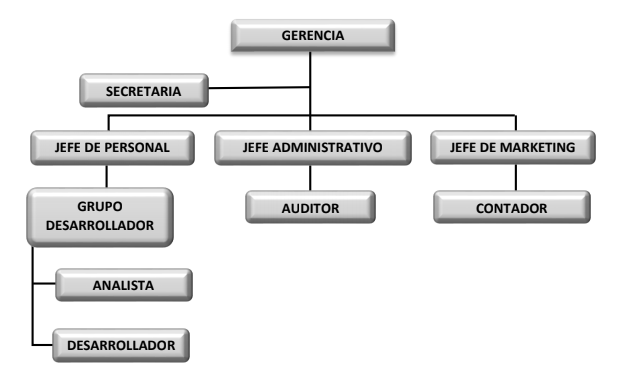
\includegraphics[width=1.2\linewidth]{libro/capitulo1/img/EstOrgSofBORe.PNG}
	\caption{Estructura Organizacional SofBORe}
\end{figure}

\section{Estructura Funcional}

\begin{figure}[htb]
	\centering
	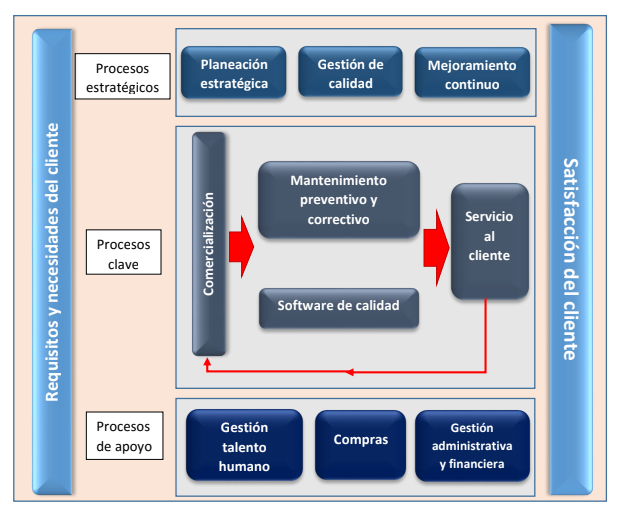
\includegraphics[width=1.0\linewidth]{libro/capitulo1/img/ProcesosSofBORe.PNG}
	\caption{Modelo de Procesos SofBORe}
\end{figure}
